% Versao em portugues para revisao; a submissao do evento exige ingles.
\PassOptionsToPackage{brazilian}{babel}
\documentclass[9pt,twocolumn,twoside,lineno]{MSBJournal}
\usepackage{etoolbox}
\renewcommand{\keywordname}{\textbf{Palavras-chave:}}
\patchcmd{\abscontent}{Abstract}{Resumo}{}{\PackageError{traducao}{Cabecalho do resumo nao encontrado}{}}
\AtBeginDocument{\selectlanguage{brazilian}\renewcommand{\refname}{Referências}}
\articletype{art}
\confyear{2026}
\confname{VI Simpósio Baiano de Modelagem e Simulação de Biossistemas}
\confdoi{Não atribuído}
\recdate{Não submetido}
\revdate{Não se aplica}
\accdate{Não aceito}
\runningtitle{Classificação de sopros cardíacos no RP2040}
\runningauthor{Santos --- rascunho de pesquisa}
\title{Classificação de sopros cardíacos com TinyML em um microcontrolador RP2040 com recursos limitados}
% TODO: confirmar autores, ordem, afiliacoes, email e ORCID.
\author[1,$\ast$]{Leandro Alves dos Santos}
\affil[1]{Universidade do Estado da Bahia (UNEB), Brasil}
\correspondingauthoraffiliation[$\ast$]{Autor correspondente: Leandro Alves dos Santos. E-mail: [A INFORMAR]. ORCID: [A INFORMAR].}
\begin{abstract}
A classificação de sopros cardíacos em microcontroladores exige avaliar conjuntamente desempenho preditivo e consumo de recursos. Treinamos uma rede neural convolucional compacta com a versão 1.0.3 da base CirCor DigiScope, considerando sopro presente e ausente. Identidades vinculadas pelos metadados e gravações idênticas foram agrupadas antes da divisão dos dados. A rede de 1.282 parâmetros processa energias logarítmicas de filtros mel em janelas de três segundos e foi quantizada para inteiros de oito bits (INT8). A reprodução digital na BitDogLab RP2040, a 133 MHz, avaliou todas as 6.512 janelas de teste, provenientes de 471 gravações e 122 grupos. Na placa, F1 foi 0,694, sensibilidade 0,708 e acurácia 0,877; o intervalo de 95\% para F1, por bootstrap de grupos, foi 0,526--0,829. Todas as decisões por grupo coincidiram com o interpretador de referência; uma diferiu da avaliação INT8 original otimizada, cujo F1 foi 0,680. Houve divergências no checksum das características em 86 janelas e nas probabilidades em 160, com diferença máxima de 0,0078125 contra a referência. Portanto, concordância de decisões não significa equivalência bit a bit. O modelo ocupou 5.264 bytes, a imagem do firmware 189.408 bytes e o espaço estático principal de SRAM 186.224 bytes. A mediana de extração de características e inferência foi 1,318 segundo. Pico de RAM, aquisição acústica, operação contínua e generalização clínica permanecem sem validação.
\end{abstract}
\keywords{TinyML; sopro cardíaco; fonocardiograma; RP2040; inferência embarcada}
\newcommand{\pending}{\textit{Pendente}}

% Guarda de limite: descarrega os floats e verifica o total real de paginas.
% A pagina seguinte e N+1 apos clearpage; valor maior que 7 significa N>6.
\AtEndDocument{%
  \clearpage
  \ifnum\value{page}>7\relax
    \PackageError{SBMSB-page-limit}{Manuscript has \number\numexpr\value{page}-1\relax\space pages; maximum is 6}{Reduce content or float size without changing the official template.}%
  \fi
}

\begin{document}
\maketitle\thispagestyle{firststyle}\slugnote\vspace{-13pt}
\noindent\textbf{Versão em português para revisão, 27 de outubro de 2026.} A versão de submissão deve ser escrita em inglês. Os resultados são os mesmos do artigo em inglês; esta tradução não representa outro experimento.

\section{Introdução}
O projeto foi desenvolvido durante as aulas de Introdução à Inteligência Artificial. Um heart murmur é um som adicional associado ao fluxo sanguíneo; pode ser inocente e não equivale, por si só, a diagnóstico de doença \citep{aha_murmurs}.
Fonocardiogramas (PCGs) representam sons cardíacos como sinais acústicos amostrados. A classificação automática de sopros tem sido investigada com gravações de diferentes focos de ausculta \citep{oliveira2022circor,reyna2023challenge}. Presença de sopro e desfecho clínico são alvos distintos: detectar um sopro não equivale a diagnosticar uma doença. Este trabalho aborda somente a presença de sopro.

A execução em microcontroladores exige mais que um arquivo de modelo pequeno. Sinal de entrada, extração de características, ativações, estruturas do interpretador e aplicação compartilham recursos limitados. TensorFlow Lite for Microcontrollers (TFLM) oferece inferência embarcada \citep{david2021tflm}, mas a viabilidade depende do processamento completo e da implementação na placa.

Investigamos o desempenho preditivo e os recursos exigidos por uma rede neural convolucional (CNN) compacta quantizada para inteiros de oito bits (INT8), executada na BitDogLab com RP2040. A contribuição combina separação por grupos, avaliação por paciente e medições no hardware, distinguindo concordância de decisões, equivalência numérica e operação acústica autônoma. A Figura~\ref{fig:pipeline} resume o fluxo experimental concluído.
\begin{figure*}[t]
\centering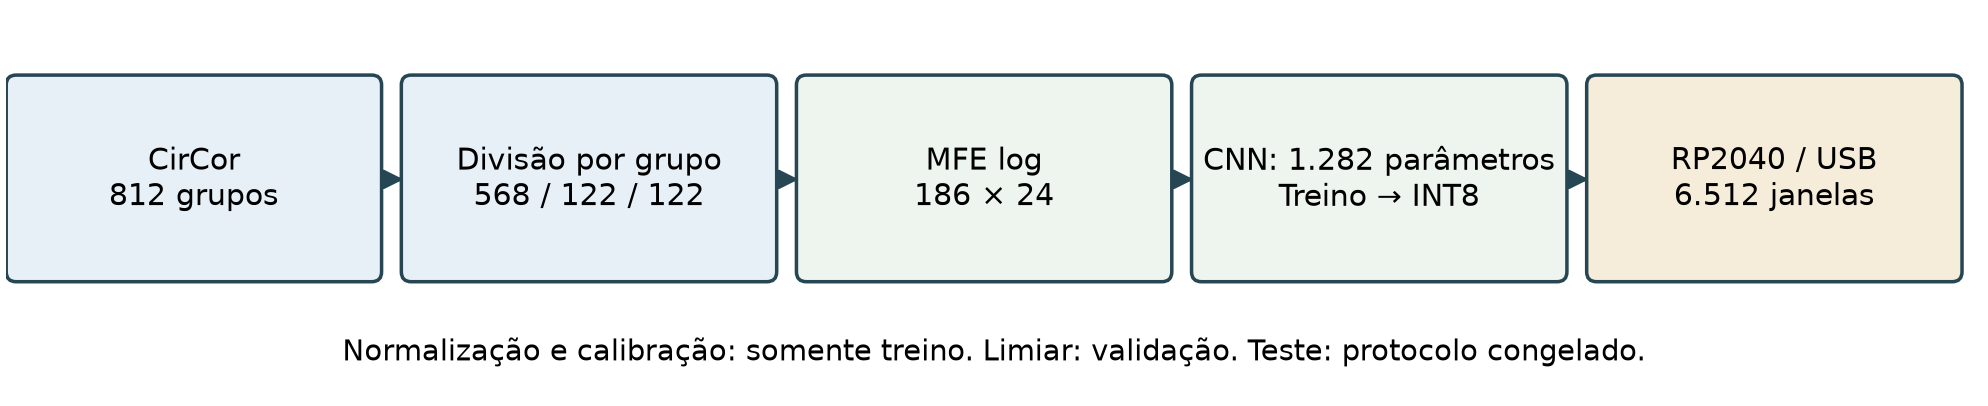
\includegraphics[width=\textwidth]{images/pipeline_pt.png}
\caption{Fluxo experimental. A divisão precede a segmentação e o ajuste da normalização. Modelo e limiares usam validação; a placa executa o modelo INT8 congelado sobre entradas digitais do teste.}
\label{fig:pipeline}
\end{figure*}

\section{Trabalhos relacionados}
A base CirCor DigiScope reúne PCGs e anotações de sopro \citep{oliveira2022circor,circor103}. O PhysioNet Challenge 2022 avaliou separadamente detecção de sopro e predição de desfecho, incluindo uma categoria de sopro desconhecido \citep{reyna2023challenge}. A exclusão dessa categoria em nosso problema binário impede a comparação direta com classificações e métricas triclasse do Challenge.

\citet{elola2023grading} combinaram espectrogramas mel, um conjunto de CNNs residuais e agregação por paciente para distinguir sopros ausentes, suaves e intensos. Isso fundamenta a investigação de representações espectrais e agregação de múltiplos focos, mas o alvo, a escala do modelo e a avaliação diferem dos nossos. Seus resultados não são usados como comparação controlada nem como evidência de execução em microcontrolador.

TFLM permite inferência em dispositivos com memória restrita \citep{david2021tflm}. A especificação de quantização define escalas, pontos zero e operações \citep{int8spec}, mas a concordância numérica depende dos kernels e do processamento de entrada. Por isso, separamos as métricas do interpretador otimizado, a referência e a execução na placa.

\section{Materiais e métodos}
\subsection{Base e divisão por grupos}
Utilizamos CirCor DigiScope 1.0.3, distribuída pelo PhysioNet \citep{circor103,pollard_physionet_2026}. Foram mantidos somente os rótulos \texttt{Murmur = Present} e \texttt{Murmur = Absent}; \texttt{Outcome} não definiu o alvo. O inventário registra 68 entradas de encontros excluídas por rótulo desconhecido/ausente e 31 entradas de gravações excluídas por conflitos em grupos vinculados. Essas contagens possuem unidades diferentes e não correspondem à soma de pessoas excluídas.

Encontros foram vinculados por metadados de identidade adicional e hashes SHA256 de WAVs idênticos. Os grupos foram distribuídos antes da segmentação, aproximadamente em 70/15/15\%, com estratificação e semente 42. Foram verificadas a separação de identificadores de grupo, encontro e gravação e a ausência de hashes compartilhados entre partições. Isso reduz vazamentos conhecidos, mas não elimina a possibilidade de identidades repetidas sem vínculo anotado. Empregamos a expressão grupos de pacientes com essa ressalva.

A coorte elegível contém 812 grupos e 2.976 gravações (Tabela~\ref{tab:split}), produzindo 28.340 janelas de treino, 6.154 de validação e 6.512 de teste. Cada janela herda o rótulo do grupo, mesmo quando um foco não apresenta sopro audível. Trata-se de supervisão fraca, sem verdade de referência acústica por janela.
\begin{table}[t]\centering
\caption{Partições obtidas. P/A: grupos com sopro presente/ausente.}\label{tab:split}
\begin{tabular}{lrrrr}\toprule
Partição & Grupos & P & A & Gravações\\\midrule
Treino & 568 & 109 & 459 & 2.066\\
Validação & 122 & 24 & 98 & 439\\
Teste & 122 & 24 & 98 & 471\\\bottomrule
\end{tabular}\end{table}
No teste, houve de uma a nove gravações por grupo, mediana quatro. As contagens por foco foram 119 aórticas (AV), 113 pulmonares (PV), 110 tricúspides (TV), 126 mitrais (MV) e três com rótulo \texttt{Phc}, mantidas sem interpretação anatômica adicional. Essas contagens não representam sopros audíveis anotados independentemente.

\subsection{Processamento do sinal}
O carregador exige áudio mono PCM16 e permite reamostragem; todas as gravações mantidas já estavam a 4 kHz. As janelas têm três segundos (12.000 amostras), com deslocamento de 1,5 s. Gravações curtas recebem zeros; caudas incompletas de gravações longas são descartadas. Remove-se a componente contínua por janela.

O processamento usa Hann periódica de 128 amostras, deslocamento de 64, espectro de potência não normalizado e 24 filtros mel triangulares de 30--1.800 Hz. Bins positivos não são duplicados. As energias logarítmicas mel (MFE) são $\log(\max(E,10^{-6}))$, formando uma matriz $186\times24$. Média e desvio por banda são ajustados somente no treino e congelados. O processamento de entrada permanece em ponto flutuante; INT8 descreve os tensores da rede. Python e C++ compartilham coeficientes e regras de preenchimento, organização e arredondamento, cuja concordância observada é avaliada separadamente.

A Figura~\ref{fig:examples} apresenta exemplos reais da validação. Selecionou-se o primeiro identificador de gravação de cada classe, independentemente da predição.
\begin{figure*}[t]\centering
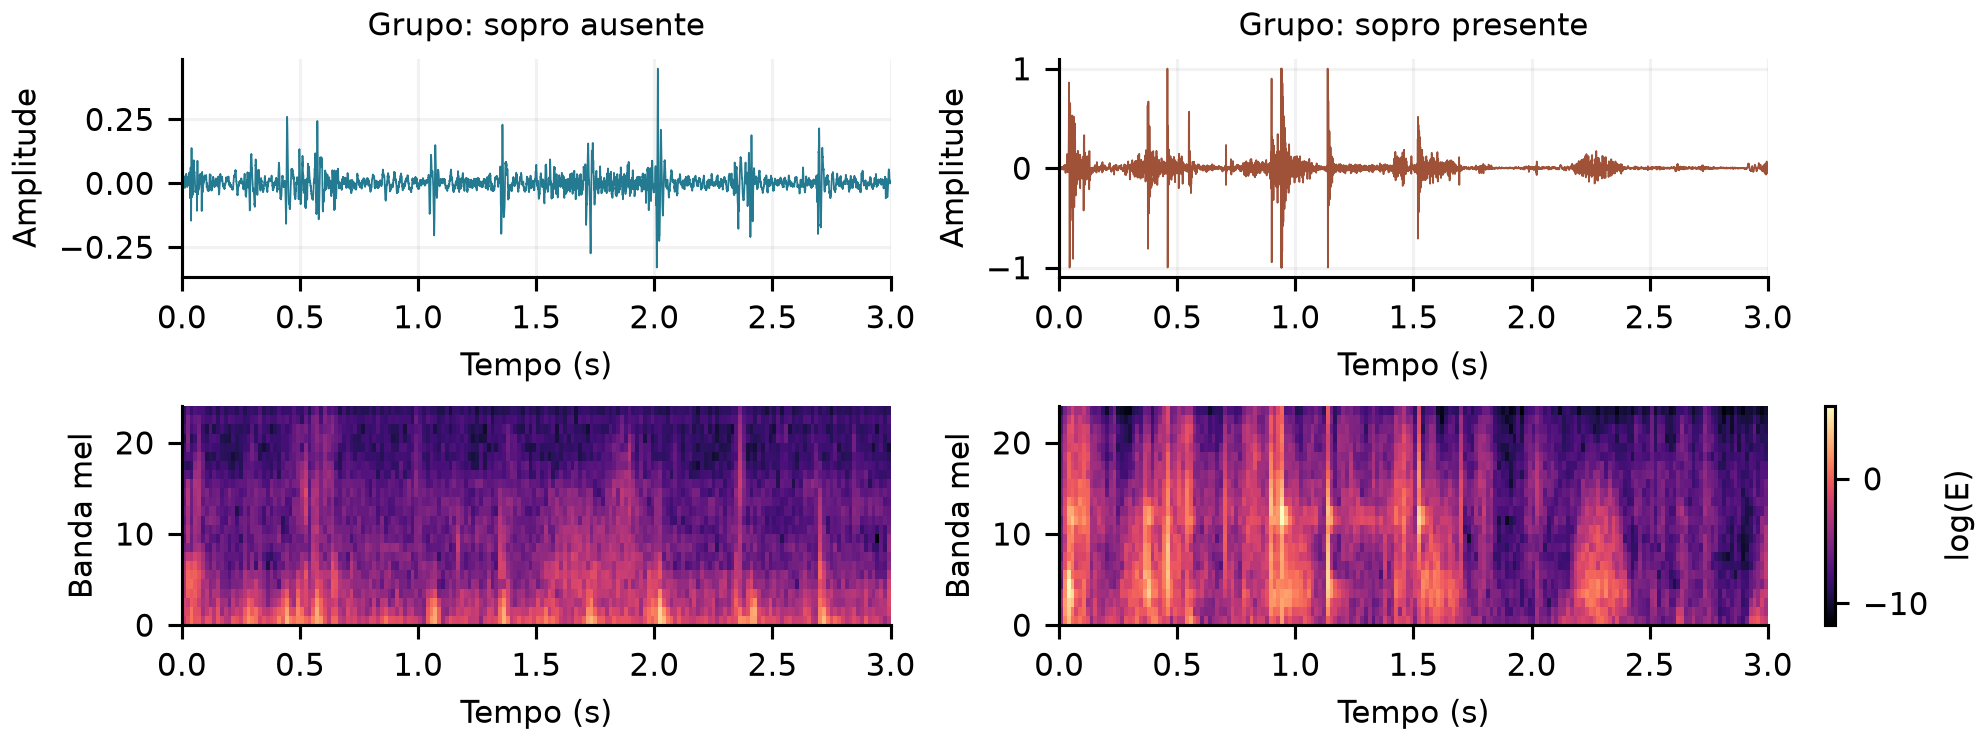
\includegraphics[width=\textwidth]{images/pcg_mfe_pt.png}
\caption{Trechos reais de três segundos da validação e MFE correspondentes da CirCor DigiScope 1.0.3 \citep{circor103}. Os títulos indicam rótulos herdados do grupo, sem confirmar sopro audível na janela. As imagens espectrais compartilham escala de cores; os eixos de amplitude das formas de onda possuem escalas próprias.}
\label{fig:examples}\end{figure*}

% Equacoes correspondentes a implementacao congelada; sem novos ajustes.
Para $x[n]$ com componente DC removida e janela Hann $w[n]=0.5-0.5\cos(2\pi n/128)$,
\begin{align}
X_t[k]&=\sum_{n=0}^{127}x[64t+n]w[n]e^{-j2\pi kn/128},\\
E_{t,b}&=\sum_{k=0}^{64}H_b[k]|X_t[k]|^2,\\
z_{t,b}&=(\log(\max(E_{t,b},10^{-6}))-\mu_b)/\sigma_b.
\end{align}
Os 24 filtros usam $m(f)=2595\log_{10}(1+f/700)$; $\mu_b$ e $\sigma_b$ provêm apenas de training. São $1+\lfloor(12000-128)/64\rfloor=186$ frames e 4.464 features.

\subsection{Rede e treinamento offline}
A CNN possui convoluções $3\times3$ com 8 e 16 canais, cada uma seguida de ativação linear retificada (ReLU) e max pooling $2\times2$, além de média global e saída softmax de duas classes. As convoluções usam preenchimento \textit{same} e passo unitário; pooling usa \textit{valid} e passo dois. O modelo tem 1.282 parâmetros treináveis.

Empregou-se Adam com taxa $10^{-3}$, lotes de 32 e no máximo 100 épocas, encerrando após dez épocas sem aumento estrito do F1 por grupo na validação. A entropia cruzada ponderou cada janela proporcionalmente a $1/(N_cW_i)$, com $N_c$ grupos da classe e $W_i$ janelas do grupo, normalizando pesos para média um. Não houve aumento de dados.

Foram treinadas sementes 42, 43 e 44. Os melhores checkpoints tiveram F1 de validação 0,451, 0,711 e 0,618; selecionou-se a semente 43, época 66. Esses valores são seleção de modelo, não três testes independentes. O treino ocorreu em RTX 5050, Arch Linux/WSL, TensorFlow 2.21, Python 3.12.15, NumPy 2.0.2 e SciPy 1.15.3.

A quantização pós-treino empregou 300 janelas de treino. O grafo convertido contém convolução, max pooling, média, camada totalmente conectada e softmax, com entrada e saída INT8, conforme a especificação \citep{int8spec}. O arquivo final ocupa 5.264 bytes. Não houve busca de arquiteturas ou ablação; o modelo não representa uma fronteira ótima entre desempenho e recursos.

Em INT8, $q=\operatorname{clip}(\operatorname{round}(z/s)+z_0,-128,127)$ e $\hat z=s(q-z_0)$. O arredondamento é feito para longe de zero em empates. No input, $(s,z_0)=(0.04310979694,-38)$; no output, $(s,z_0)=(1/256,-128)$. O tensor de input usa 4.464 bytes em INT8 ou 17.856 em Float32. Isso não implica firmware quatro vezes menor ou mais rápido. Bias e accumulators usam INT32; o MFE permanece floating point. As camadas têm 80, 1.168 e 34 parâmetros, totalizando 1.282.

\subsection{Implementação na placa}
Uma aplicação C/C++ executa MFE e TFLM na BitDogLab RP2040, alvo \texttt{pico\_w}, core 0 a 133 MHz, sem comunicação sem fio ou carga no segundo núcleo. O RP2040 possui 264 KiB de memória estática (SRAM) \citep{rp2040docs}; a revisão física da placa não foi registrada independentemente.

Usaram-se Pico SDK, commit \texttt{95ea6ac}; porte TFLM, commit \texttt{dfea53b}; Arm GNU Toolchain 14.2.Rel1; CMake 3.31.6 e Ninja 1.11.1.4. A aplicação usou \texttt{-O2}; TFLM foi otimizado para tamanho. As entradas PCM16 foram transmitidas por USB. Microfone e OLED da plataforma \citep{bitdoglab} não integraram o benchmark.

Uma demonstração OLED/RGB separada foi posteriormente compilada com duas janelas de validação armazenadas. Uma conferência funcional manual relatou alternância das saídas no OLED e das indicações verde/vermelha no LED RGB. As saídas por janela são ilustrativas e não reproduzem a agregação por paciente. Seus custos adicionais não foram medidos e não são atribuídos ao firmware do experimento.
% TODO: registrar revisao fisica e medir custos adicionais da interface separadamente.

\section{Configuração experimental}
\subsection{Agregação e métricas}
Calcula-se a média das probabilidades das janelas por gravação; o escore do grupo é o máximo entre gravações. O limiar maximiza F1 na validação, com desempate por maior sensibilidade e menor limiar. Os limiares float e INT8 são 0,725111204844 e 0,734675480769, respectivamente; o segundo permaneceu fixo na placa. Quantidade de gravações e cobertura de focos podem influenciar a agregação pelo máximo.

Compararam-se preditor da classe majoritária do treino, CNN float e CNN INT8 nos mesmos 122 grupos. A avaliação INT8 original no computador usou AUTO/XNNPACK. O alvo positivo é sopro presente, e a medida principal é
\begin{equation}
F_1=\frac{2VP}{2VP+FP+FN},\qquad R=\frac{VP}{VP+FN}.
\end{equation}
VP/VN e FP/FN representam verdadeiros e falsos positivos/negativos. Precisão, acurácia, especificidade, macro-F1 e contagens de confusão complementam F1. Intervalos percentis de 95\% foram obtidos por bootstrap ordinário de grupos, com 2.000 replicações e semente 2026. O teste não selecionou modelos, agregação ou limiares.

\subsection{Paridade, memória e tempo}
Dez gravações de validação, cinco por classe, compararam processamento e inferência antes do teste completo. O diagnóstico encontrou features INT8 exatas, mas diferenças de até 0,015625 contra AUTO/XNNPACK. O resolvedor de comparação foi então alterado para LiteRT 2.3.0 \texttt{BUILTIN\_REF}, preservando pesos, limiares e tolerâncias. Essa revisão posterior ao diagnóstico ocorreu na validação e manteve os resultados originais do host. O critério admite até um passo de entrada e dois de saída. A compatibilidade com kernels inteiros de referência é uma questão documentada para Arm \citep{cmsisnn}.

Um benchmark separado reproduziu a primeira janela de 100 gravações da validação embaralhadas com semente 2026, após dez aquecimentos. O temporizador \texttt{time\_us\_64} mediu processamento e inferência; aquisição, USB, CRC, display e inicialização ficaram fora. O tamanho de flash foi obtido da imagem binária e a memória estática das seções ELF. Ocupação da arena difere de capacidade; pico de RAM e uso máximo de pilha não foram instrumentados.

\subsection{Teste completo na placa}
O protocolo congelado cobriu 6.512 janelas, 471 gravações e 122 grupos. As respostas foram preservadas em diário com cadeia de hashes. Um timeout de escrita USB interrompeu a primeira sessão após 1.293 janelas; as 5.219 restantes foram coletadas na retomada, com o mesmo modelo, fontes e protocolo. A causa física não foi determinada.

Métricas foram liberadas somente após concluir a coorte. Uma auditoria offline verificou a cadeia e hashes dos artefatos e recalculou agregação, métricas e intervalo principal. Todas as janelas foram incluídas; discordâncias não levaram a exclusões ou ajustes.

\section{Resultados e discussão}
\subsection{Desempenho entre interpretadores}
A Tabela~\ref{tab:predictive} mostra as avaliações concluídas. Na placa, F1 foi 0,694 (IC95\% 0,526--0,829), sensibilidade 0,708 (17/24 positivos), precisão 0,680 e especificidade 0,918. O resultado INT8 original otimizado permanece 0,680 (IC95\% 0,512--0,816). Placa e referência coincidem nas 122 decisões; o host otimizado difere em um grupo negativo, com nove falsos positivos em vez de oito (Tabela~\ref{tab:confusion}).

Float e INT8 na placa possuem as mesmas contagens, o que não implica probabilidades iguais. As diferenças envolvem processamento de entrada e kernels; não isolam uma causa nem comprovam melhoria do modelo pelo hardware. A pequena coorte positiva produz intervalos amplos.
\begin{table}[t]\centering\setlength{\tabcolsep}{4pt}
\caption{Resultados em 122 grupos. Opt./ref.: kernels otimizados/de referência. R: sensibilidade; Acc.: acurácia.}\label{tab:predictive}
\begin{tabular}{lrrrr}\toprule
Execução & F1 & R & Acc. & Macro-F1\\\midrule
Sempre ausente & 0,000 & 0,000 & 0,803 & 0,445\\
CNN float & 0,694 & 0,708 & 0,877 & 0,808\\
INT8 host (opt.) & 0,680 & 0,708 & 0,869 & 0,799\\
INT8 host (ref.) & 0,694 & 0,708 & 0,877 & 0,808\\
INT8 RP2040 & 0,694 & 0,708 & 0,877 & 0,808\\\bottomrule
\end{tabular}\end{table}
\begin{table}[t]\centering
\caption{Contagens de confusão; sopro presente é positivo.}\label{tab:confusion}
\begin{tabular}{lrrrr}\toprule
Execução & VP & FN & FP & VN\\\midrule
Sempre ausente & 0 & 24 & 0 & 98\\
CNN float & 17 & 7 & 8 & 90\\
INT8 host (opt.) & 17 & 7 & 9 & 89\\
INT8 host (ref.) & 17 & 7 & 8 & 90\\
INT8 RP2040 & 17 & 7 & 8 & 90\\\bottomrule
\end{tabular}\end{table}
O preditor majoritário tem acurácia de 80,3\%, sem detectar positivos e com precisão indefinida. A rede ainda não detecta sete de 24 grupos positivos. Exclusão de unknown, supervisão fraca e ausência de validação externa limitam a interpretação clínica. Trata-se de protótipo de pesquisa.

A Figura~\ref{fig:results} reúne matriz de confusão, incerteza do F1 e custos de processamento. Os intervalos usam grupos como unidade, enquanto os tempos abrangem as 6.512 janelas.
\begin{figure*}[t]\centering
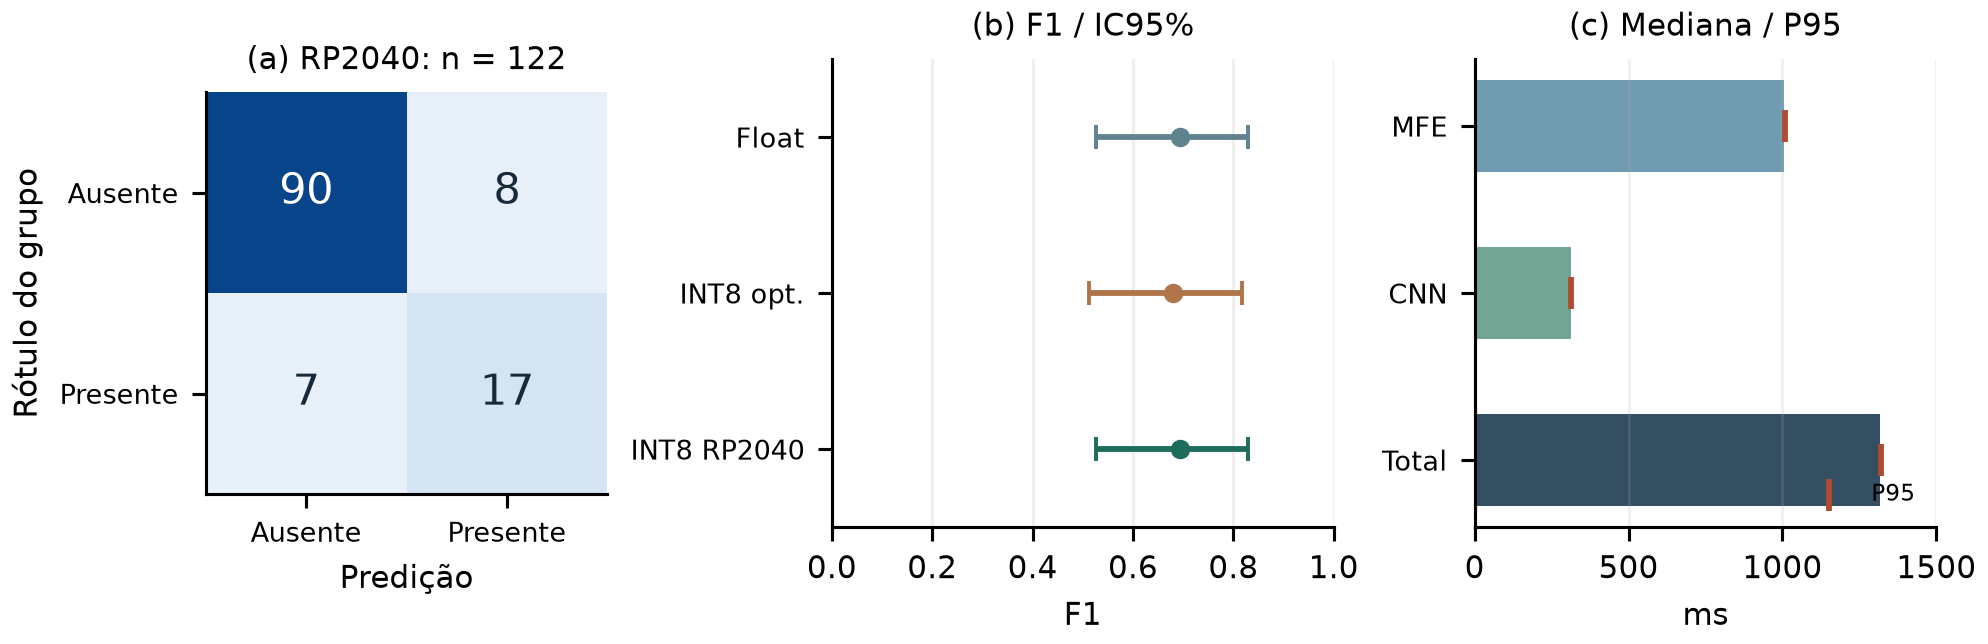
\includegraphics[width=\textwidth]{images/results_pt.png}
\caption{Teste completo: (a) confusão na placa para 122 grupos; (b) F1 e intervalos de 95\% por bootstrap de grupos; (c) mediana de tempo, com marcadores P95. Tempos excluem aquisição, USB, CRC, display e inicialização.}
\label{fig:results}\end{figure*}

\subsection{Recursos na placa}
A Tabela~\ref{tab:resources} distingue armazenamento e memória. A ocupação de 46.100 bytes está contida na reserva de 147.456 bytes da arena e não deve ser somada novamente. O espaço estático de 186.224 bytes inclui código/dados copiados, vetores, BSS e alinhamento; exclui reservas de heap e pilhas e não é pico de uso. Há reserva mínima de heap de 2.048 bytes e de 4.096 bytes para a pilha de cada núcleo, embora o segundo não execute a aplicação.
\begin{table}[t]\centering
\caption{Recursos na placa, em bytes.}\label{tab:resources}
\begin{tabular}{p{0.66\columnwidth}r}\toprule
Quantidade & Bytes\\\midrule
Modelo INT8 serializado & 5.264\\
Imagem flash do firmware & 189.408\\
Espaço estático principal de SRAM & 186.224\\
Capacidade da arena (já incluída) & 147.456\\
Ocupação da arena (dentro da reserva) & 46.100\\
Buffer PCM (já incluído) & 24.000\\
Pico de RAM / uso máximo da pilha & \pending\\\bottomrule
\end{tabular}\end{table}

\subsection{Concordância numérica}
Os 44.640 elementos INT8 das dez entradas de validação coincidiram exatamente, com diferença de saída zero contra a referência. No teste completo, 86/6.512 janelas (1,32\%) apresentaram checksums CRC32 distintos nas features quantizadas. Não foram preservados tensores completos dessas entradas na placa; a causa e a magnitude por elemento não podem ser estabelecidas pelo diário. Divergência de CRC de features não comprova corrupção do pacote USB.

As probabilidades diferiram da referência em 160 janelas, com máximo de 0,0078125, dois passos de quantização da saída. Mesmo assim, todas as decisões por grupo coincidiram. Contra o host otimizado, a concordância foi 121/122 e a diferença máxima por janela 0,078125. Há reprodutibilidade de decisões neste teste, sem equivalência numérica completa. As diferenças foram mantidas como limitação, sem correção baseada no teste.
% TODO: investigar diferencas em protocolo separado, sem ajustar ao teste.

\subsection{Latência no teste completo}
A Tabela~\ref{tab:timing} contém tempos das 6.512 janelas, excluindo validação e aquecimento repetidos no início de cada sessão. A mediana de MFE foi 1.006,536 ms e a de inferência 311,868 ms; o processamento de entrada domina o custo. O máximo combinado, 1.323,475 ms, ficou abaixo do deslocamento de 1.500 ms. Isso não demonstra operação contínua, pois aquisição e outros custos foram excluídos. Não houve medição float na placa para quantificar ganho de velocidade por INT8.
\begin{table}[t]\centering\setlength{\tabcolsep}{4pt}
\caption{Latência do teste completo, 6.512 janelas, em milissegundos.}\label{tab:timing}
\begin{tabular}{lrrr}\toprule
Etapa & Mediana & P95 & Máximo\\\midrule
MFE & 1.006,536 & 1.008,025 & 1.011,607\\
Inferência & 311,868 & 311,884 & 312,178\\
Combinado & 1.318,405 & 1.319,889 & 1.323,475\\\bottomrule
\end{tabular}\end{table}
% TODO: instrumentar pico de RAM e uso de pilha em experimento separado.

\subsection{Benchmark suplementar de CPU, RTX e INT8}
Em sessão separada de 27/10, repetiram-se as mesmas 100 janelas de validation do benchmark anterior: dez warm-up calls excluídas, três repetições e batch size um. CPU/RTX Float32 usaram TensorFlow 2.21 com leitura sincronizada do output, excluindo criação/upload do input; MFE permaneceu na CPU. Float32/INT8 na CPU usaram TFLite 2.21 \texttt{BUILTIN\_REF}, uma thread e tempo de Invoke. A placa executou a demonstração V3 auditada a 133 MHz, diferente do firmware da Tabela~\ref{tab:resources}.
\begin{table}[t]\centering
\caption{Benchmark suplementar: 300 chamadas por modo, medianas em ms.}\label{tab:fresh}
\begin{tabular}{lrr}\toprule
Execução & Inference & MFE + rede\\\midrule
CPU Float32 (TF) & 0,661 & 0,836\\
RTX Float32 (TF) & 0,768 & 0,956\\
CPU Float32 (ref.) & 1,347 & 1,509\\
CPU INT8 (ref.) & 1,932 & 2,113\\
RP2040 INT8 (V3) & 312,077 & 1.322,608\\\bottomrule
\end{tabular}\end{table}
O TFLite Float32 ocupou 7.984 bytes contra 5.264 em INT8 (redução de 34,1\%); a conversão concordou com a saída do modelo CPU até $4,77\times10^{-7}$. INT8 não reduziu a latência no reference kernel de CPU. A diferença média absoluta dos window scores Float32/INT8 foi 0,01454, com duas decisões diferentes em cem usando o mesmo threshold INT8. Isso não é accuracy por paciente. Placa e CPU INT8 tiveram os mesmos scores nas cem janelas. A RTX não reduziu a latência individual nesta sessão; dispatch/readback é uma hipótese não isolada. Janelas correlacionadas, ordem fixa dos modos e escopos de tempo distintos limitam conclusões sobre hardware. Não houve novo training, ajuste de threshold ou substituição dos resultados do test set.

\subsection{Reprodutibilidade e evidências restantes}
Foram preservados inventário, manifesto de grupos, históricos de treino, recibo de exportação, predições originais, auditoria do binário e diários USB. O modelo tem prefixo SHA256 \texttt{3b7e258e26ca}; recibos contêm o digest completo e hashes das fontes. Os diários brutos permanecem locais; código, evidências curadas e materiais didáticos estão em \url{https://github.com/Lawtrel/bitdoglab-heart-tinyml}. Não foram adquiridas novas gravações de participantes.

Avaliação original no host, benchmark de validação e teste completo na placa são evidências fixadas. A retomada preservou pesos, limiares, ordem e tolerâncias. Experimentos acústicos, diagnósticos numéricos e memória exigem configurações separadas. Não houve mudanças de modelo, agregação ou limiar a partir do teste concluído.

\section{Conclusão}
Uma CNN de 1.282 parâmetros, quantizada em um modelo de 5.264 bytes, obteve F1 de 0,694, sensibilidade 0,708 e acurácia 0,877 na reprodução completa do teste na BitDogLab RP2040. As decisões coincidiram com a referência nos 122 grupos, mas diferenças nas features e probabilidades impedem alegar equivalência bit a bit. A mediana combinada de 1,318 segundo sustenta viabilidade de reprodução digital controlada. Incerteza ampla, diferenças numéricas não resolvidas, pico de RAM não medido e ausência de validação acústica/contínua limitam o resultado. Esses pontos devem ser investigados em experimentos separados, sem reajustar o modelo pelo teste.

\bibliographystyle{abbrvnat}\bibliography{references}
\end{document}

